\section*{Dati e risultati}

\subsection*{Rilevatore di picchi}

Dopo aver costruito il circuito mostrato nello schema (a), abbiamo studiato il circuito in funzione della capacità
$C$ e della resistenza $R_1$. Abbiamo quindi misurato la tensione $V\ped{out}$ variando $C$ e mantenedo $R_1 = \SI{1}{\kilo\ohm}$.
In seguito è stata misurata la $V\ped{out}$ mantenendo $C = \SI{1}{\micro\farad}$ e variando $R_1$.
In entrambi i casi il circuito è stato alimentato con onde quadre di frequenza \SI{1}{\kilo\hertz}

\begin{SCfigure}
    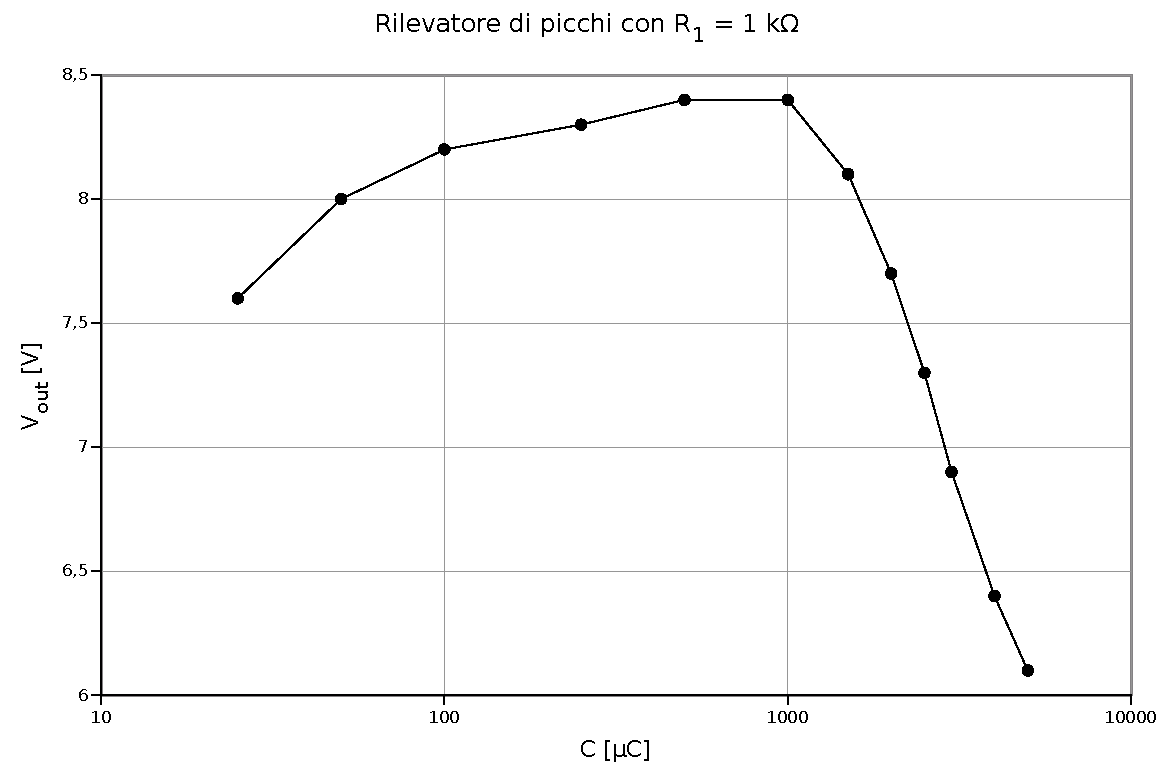
\includegraphics[scale=0.7]{capacita.pdf}
    \caption{}
    \label{fig:capacita}
\end{SCfigure}

\begin{SCfigure}
    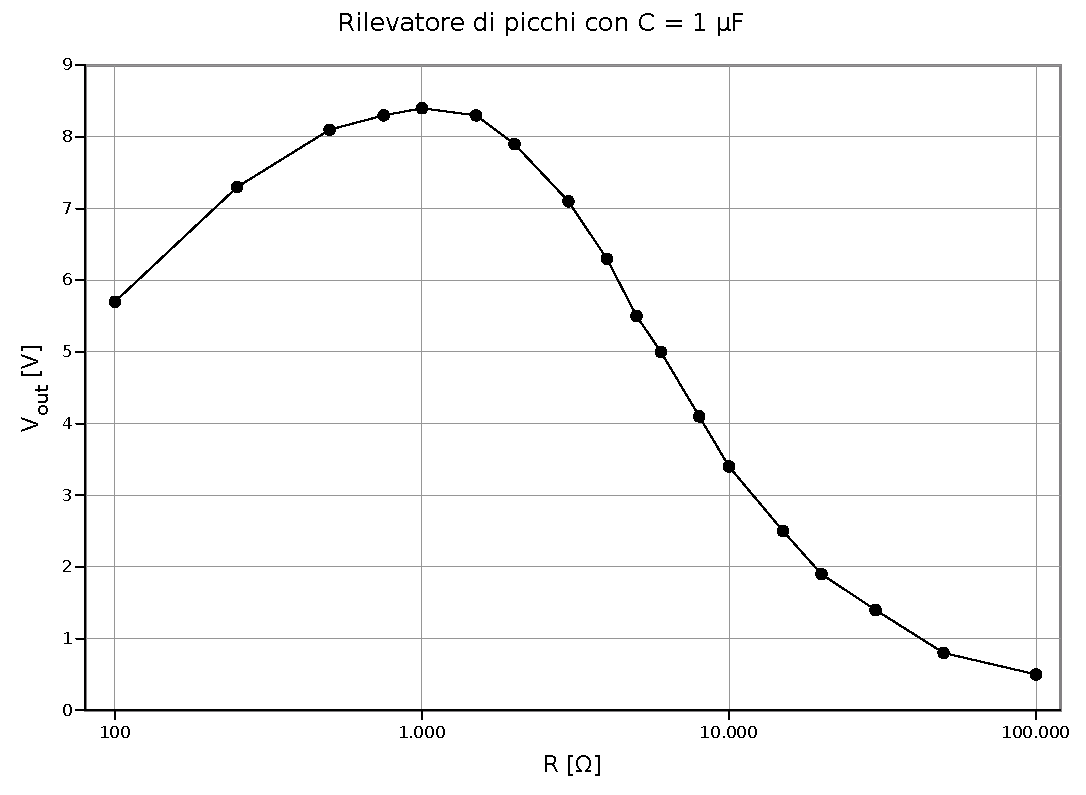
\includegraphics[scale=0.7]{resistenza.pdf}
    \caption{Andrea è un party dancer. Sono un fucking spammer.}
    \label{fig:resistenza}
\end{SCfigure}

\begin{SCfigure}
    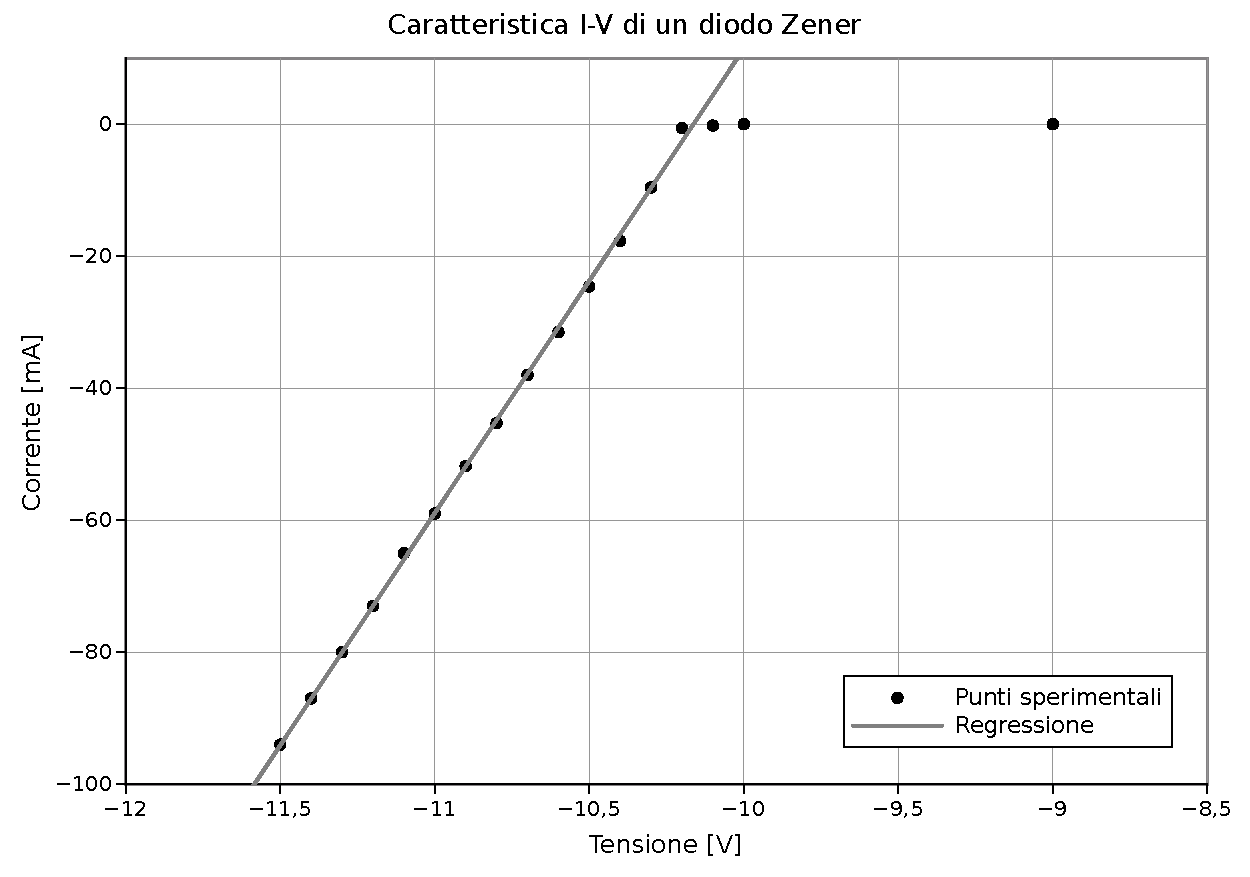
\includegraphics[scale=0.7]{cara_zener.pdf}
    \caption{Andrea è un party dancer. Sono un fucking spammer.}
    \label{fig:resistenza}
\end{SCfigure}

\begin{SCfigure}
    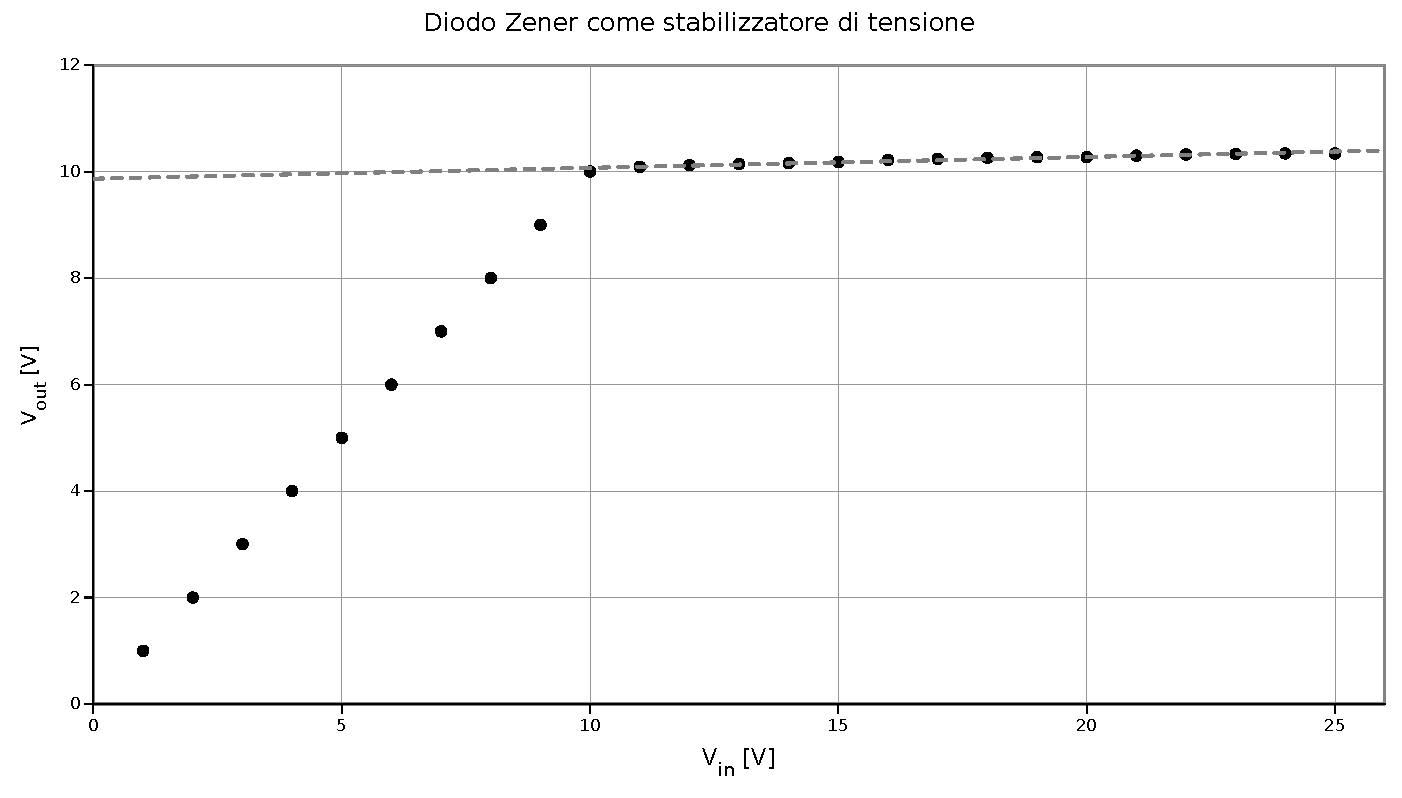
\includegraphics[scale=0.7]{stab.pdf}
    \caption{Andrea è un party dancer. Sono un fucking spammer.}
    \label{fig:resistenza}
\end{SCfigure}
